\section{LSST Image Processing Steps and Data Products Relevant for Asteroids} \label{sec:AppA}

The data products produced by the LSST Data Management system are described in 
LSST Document LSE-163\footnote{See http://ls.st/LSE-163} (LSST Data Products
Definition Document). Here we briefly summarize parts of that
document\footnote{To ensure the continued scientific adequacy of LSST data 
products, their designs and plans are periodically reviewed and updated and
thus LSE-163 is a living document -- please always consult the latest version.}
that are most relevant for discovering moving Solar System objects. 

LSST Data Management system will perform nightly analysis of difference images\footnote{A difference
image is an image produced by subtracting a science image from an appropriate 
``average'' of the previously collected similar images of the same sky area, and using the 
same filter.}, with the goal of detecting and characterizing astrophysical phenomena 
revealed by their time-dependent nature. The detection of supernovae superimposed 
on bright extended galaxies is an example of this analysis, and of course moving Solar
System objects are another example. The processing will be done on nightly/daily 
basis and will result in the so-called Level 1 data products. Level 1 products will include 
difference images, catalogs of sources detected in difference images (the so-called
\DIASources), static astrophysical objects\footnote{The LSST has adopted the nomenclature by 
which single-epoch detections of astrophysical {\em objects} are called {\em sources}. 
The reader is cautioned that this nomenclature is not universal: some surveys call 
{\em detections} what LSST calls {\em sources}, and use the term {\em sources} for what 
LSST calls {\em objects}.} these \DIASources are positionally associated to (the so-called \DIAObjects), 
and moving Solar System objects (\SSObjects\footnote{\SSObjects used to be called 
``Moving Objects'' in previous versions of the LSST Data Products baseline. The name is 
potentially confusing as high-proper motion stars are moving objects as well. A more 
accurate distinction is the one between objects {\em inside} and {\em outside} of the Solar 
System.}). The catalogs will be entered into the Level 1 database and made available in near 
real time. Notifications (``alerts'') about new \DIASources will be issued using 
community-accepted standards\footnote{For example, VOEvent, see http://ls.st/4tt} within 
60 seconds of observation. 

Moving Object Processing Software (\code{MOPS}) pipeline  combines all unassociated \DIASources into 
plausible \SSObjects and estimates their orbital parameters. The three main pipeline stages
include associating new \DIASources with known \SSObjects, discovering new \SSObjects, 
and orbit refinement and management. This conceptual MOPS design is illustrated in  
Figure~\ref{fig:Pipe8}. Further details about the MOPS pipeline design and implementation are available
from the LSST Science Pipelines Design Document\footnote{See http://ls.st/LDM-151}, LDM-151.
The next section briefly describes the main processing steps in nightly/daily Level 1 data processing. 

\begin{figure}[!t]
    \centering
    %\vskip -2.3in 
%    \hskip -0.2in
    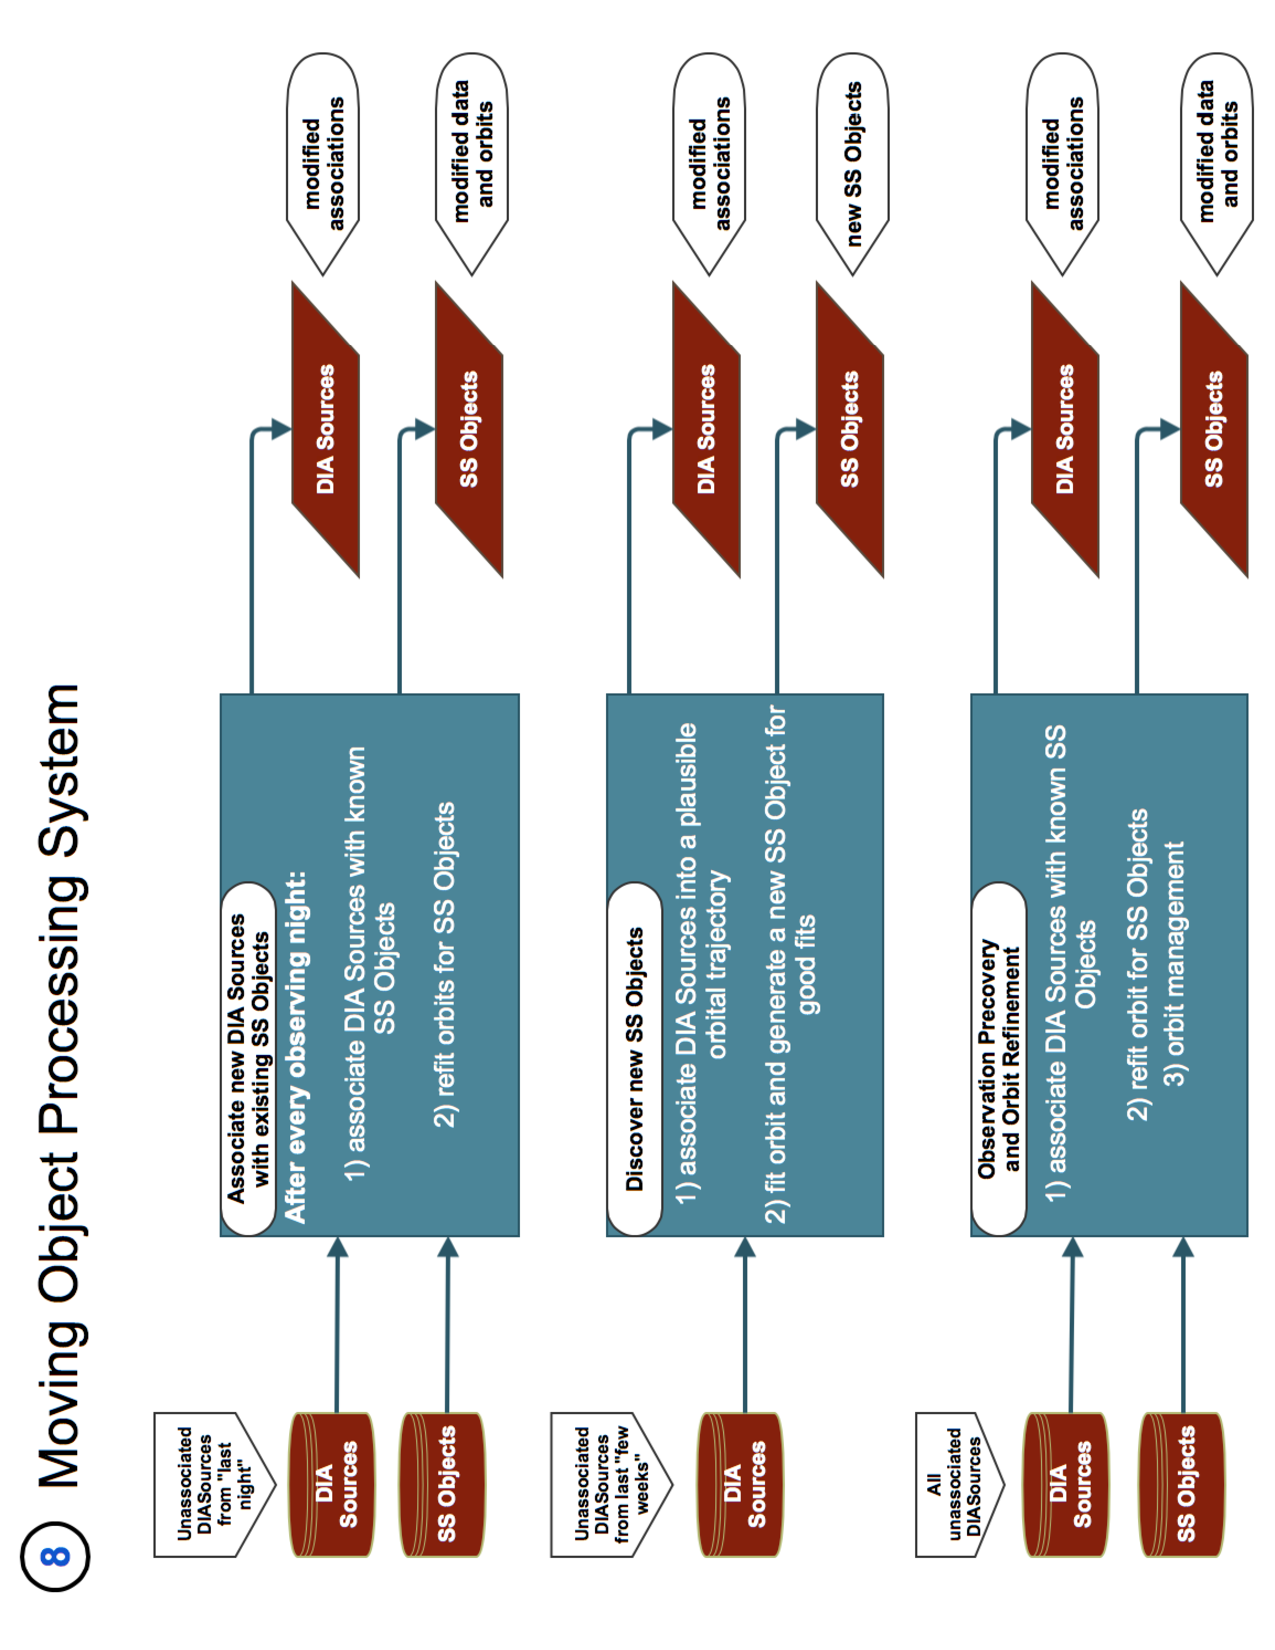
\includegraphics[scale=0.60, angle=270]{MOPS-Level0}
    \vskip -0.1in 
    \caption{Illustration of the conceptual algorithm design for the Moving Object Processing Software. 
   \DIASources are data structures that describe detections of sources in difference images and 
   \SSObjects are data structures that describe discovered Solar System objects (see Table~\ref{tab:SSObj}).
\label{fig:Pipe8}}    
\end{figure}


\subsection{LSST Level 1 Data Processing} 

Level 1 data products are a result of difference image analysis (DIA). 
\DIASources are sources detected on difference images with the signal-to-noise ratio $S/N>transSNR$, 
with $transSNR$=5. 
They represent changes in flux with respect to a deep template. Physically, a \DIASource may be an observation of new astrophysical object that was not present at that position in the template image (for example, an asteroid), or an observation of flux change in an existing source (for example, a variable star). Their flux can be negative (eg., if a source present in the template image reduced its brightness, or moved away). Their shape can be complex (eg., trailed, for a source with proper motion approaching $\sim {\rm deg}/{\rm day}$, or ``dipole-like", if an object's observed position exhibits an offset -- true or apparent -- compared to its position on the template). 
Some \DIASources will be caused by background fluctuations; with $transSNR = 5$, 
the expected false positive rate is about one per CCD (XX per sq. deg. for the median seeing, 
or of the order 200,000 per typical night). 
The expected number of false positives due to background fluctuations is a very strong function 
of adopted $transSNR$: a change of $transSNR$ by 0.5
results in a variation of an order of magnitude, and a change of $transSNR$ by unity changes the number of false
positives by about two orders of magnitude.

Clusters of \DIASources detected on visits taken at different times are associated with either a \DIAObject or an \SSObject, to represent the underlying astrophysical phenomenon. The association can be made in two different ways: by assuming the underlying phenomenon is an object within the Solar System moving on an orbit around the Sun\footnote{LSST pipelines will not fit for motion around other Solar System bodies; eg., identifying new satellites of Jupiter is left to the community.}, or by assuming it to be distant enough to only exhibit small parallactic and proper motion\footnote{Where 'small' is small enough to unambiguously positionally associate together individual apparitions of the object.}. The latter type of association is performed during difference image analysis right after the image has been acquired. The former is done at daytime by \code{MOPS}, unless the \DIASource is an apparition of an already known \SSObject. In that case, it will be flagged as such during difference image analysis. At the end of the difference image analysis of each visit, LSST will issue time domain event alerts for all 
newly detected \DIASources\footnote{For observations on the Ecliptic near the opposition Solar System objects will dominate the \DIASource counts and (until they're recognized as such) overwhelm the explosive transient signal. It will therefore be advantageous to quickly identify the majority of Solar System objects early in the survey.}.

The following is a high-level description of steps which will occur during regular {\em nightly} 
difference image analysis:
\begin{enumerate}
\item A visit is acquired and reduced to a single {\em visit image} (cosmic ray rejection, instrumental signature removal\footnote{Eg., subtraction of bias and dark frames, flat fielding, bad pixel/column interpolation, etc.}, etc.).
\item The visit image is differenced against the appropriate template and \DIASources are detected and
their properties measured. 
\item The flux and shape\footnote{The ``shape'' in this context consists of weighted 2$^{\rm nd}$ moments
of the intensity distribution, as well as fits to a trailed source model and a dipole model.} of the DIASource are measured on the difference image. PSF photometry is performed on the visit image at the position of the \DIASource to obtain a measure of the total flux.
\item The Level 1 database is searched for a \DIAObject or an \SSObject with which to positionally associate the newly discovered \DIASource\footnote{The association algorithm will guarantee that a \DIASource is associated with not more than one existing \DIAObject or \SSObject. The algorithm will take into account the parallax and proper (or Keplerian) motions, as well as the errors in estimated positions of \DIAObject, \SSObject, and \DIASource, to find the maximally likely match. Multiple \DIASources in the same visit will not be matched to the same \DIAObject.}. If no match is found, a new \DIAObject is created and the observed \DIASource is associated to it.
\item If the \DIASource has been associated with an \SSObject (a known Solar System object), it will be flagged as such and an alert will be issued. Further processing will occur in daytime (see \S\ref{sec:ssProcessing} below).
\item Otherwise, the associated \DIAObject measurements will be updated with new data 
collected during previous 12 months. All affected columns will be recomputed, including proper motions, centroids, light curves, etc.
\item The \DR\footnote{\DR is a database resulting from annual data release processing.} is searched for one or more \Objects positionally close to the \DIAObject, out to some maximum radius\footnote{Eg., a few arcseconds.}. The IDs of these nearest-neighbor \Objects are recorded in the \DIAObject record and provided in the issued 
event alert.
\item An alert is issued that includes the \DIASource ID, the \SSObject ID or \DIAObject ID, and the associated science content (centroid, fluxes, low-order lightcurve moments, periods, etc.), including the full light curves. 
\item For all \DIAObjects overlapping the field of view, including those that have an associated 
new \DIASource from this visit, forced photometry will be performed on difference image (point source photometry only). 
No alerts will be issued for these \DIASources.
\item Within 24 hours of discovery, {\em precovery} PSF forced photometry will be performed on any difference image overlapping the position of new \DIAObjects taken within the past 30 days, and added to the database. Alerts will not be issued with precovery photometry information.
\end{enumerate}

In addition to the processing described above, a smaller sample of sources detected on difference images {\em below} the nominal $transSNR = \transSNR$ threshold will be measured and stored, in order to enable monitoring of difference image analysis quality.

Also, the system will have the ability to measure and alert on a limited\footnote{It will be sized for no less than $\sim 10\%$ of average \DIASource per visit rate.} number of sources detected below the nominal threshold for which additional criteria are satisfied. For example, a $transSNR = 3$ source detection near a gravitational keyhole\footnote{
A gravitational keyhole is a region of space where Earth's gravity would modify the orbit of a passing asteroid 
such that the asteroid would collide with the Earth in the future.}
may be highly significant in assessing the danger posed by a potentially hazardous asteroid. 
The initial set of criteria will be defined by the start of LSST operations.

\subsubsection{Solar System Object Processing \label{sec:ssProcessing}} 

The following will occur during regular Solar System object processing (in daytime\footnote{Note that there {\em is no strict bound on when daytime Solar System processing must finish}, just that, averaged over some reasonable timescale (eg., a month), a night's worth of observing is processed within 24 hours. Nights rich in moving objects may take longer to process, while nights with less will finish more quickly. In other words, the system requirement is on {\em throughput}, not latency.}, after a night of observing; see Figure~\ref{fig:Pipe8}):
\begin{enumerate}
\item The orbits and physical properties of all \SSObjects re-observed on the previous night are recomputed. External orbit catalogs (or observations) are also used to improve orbit estimates. Updated data are entered to the \SSObjects table. 
\item All \DIASources detected on the previous night, that have {\em not} been matched at a high confidence level to a known \Object,
\DIAObject, \SSObject, or an artifact, are analyzed for potential pairs, forming {\em tracklets}.
\item The collection of tracklets collected over the past 30 days is searched for subsets forming {\em tracks} consistent with being on the same Keplerian orbit around the Sun.
\item For those that are, an orbit is fitted and a new \SSObject table entry created. \DIASource records are updated to point to the new \SSObject record. \DIAObjects ``orphaned'' by this unlinking are deleted.\footnote{Some \DIAObjects may only be left with forced photometry measurements at their location (since all \DIAObjects are force-photometered on previous and subsequent visits);  these will be kept but flagged as such.}.
\item Precovery linking is attempted for all \SSObjects whose orbits were updated in this process. Where successful, \SSObjects (orbits) are recomputed as needed.
\end{enumerate}


\subsubsection{Level 1 Catalogs}
\label{sec:level1db}

The described alert processing design relies on the ``living'' \DB that contains the objects and sources detected on difference images. At the very least\footnote{It will also contain exposure and visit metadata, MOPS-specific tables, etc.}, this database will have tables of \DIASources, \DIAObjects, and \SSObjects, populated in the course of nightly and daily difference image and Solar System object processing\footnote{The latter is also colloquially known as {\em DayMOPS}.}. As these get updated and added to, their updated contents becomes visible (query-able) immediately\footnote{No later than the moment of issuance of any event alert that may refer to it.}.

Table~\ref{tab:SSObj}  presents the {\em conceptual schema} for the \SSObject table (it conveys {\em what} data
will be recorded in each table, rather than the details of {\em how}). 
Columns whose type is an array will likely be expanded to one table column per element of the array
once this schema is translated to SQL\footnote{The SQL realization of this schema can be browsed at \url{http://ls.st/8g4}}. In addition, the table presented here is normalized (i.e., it contains no redundant 
information with other tables in Level 1 database). For example, since the band of observation can be found 
by joining a \DIASource table to the table with exposure metadata, there's no column named {\tt band} in the \DIASource table. In the as-built database, the views presented to the users will be appropriately denormalized 
for ease of use.

\subsubsection{\SSObject Table \label{tab:SSObj}}

\begin{center}
\label{tab:SSObj}
\begin{longtable}{p{3cm}p{2cm}p{2cm}p{5cm}}
%\caption[\SSObject Table]{\SSObject Table} \\

\hline \multicolumn{1}{c}{\bf Name} & \multicolumn{1}{c}{\bf Type} & \multicolumn{1}{c}{\bf Unit} & \multicolumn{1}{c}{\bf Description} \\ \hline
\endhead

\hline \multicolumn{4}{r}{{\em Continued on next page}} \\
\endfoot

\hline\hline
\endlastfoot

ssObjectId & uint64 & ~ & Unique identifier. \\ 

oe & double[7] & various & Osculating orbital elements at epoch ($q$, $e$, $i$, $\Omega$, $\omega$, $M_0$, epoch). \\

oeCov & double[21] & various & Covariance matrix for \texttt{oe}. \\

arc & float & days & Arc of observation. \\

orbFitLnL & float & ~ & Natural log of the likelihood of the orbital elements fit. \\

orbFitChi2 & float & ~ & $\chi^2$ statistic of the orbital elements fit. \\

orbFitNdata & int & ~ & The number of data points (observations) used to fit the orbital elements. \\

MOID & float[2] & AU & Minimum orbit intersection distances\footnote{\url{http://www2.lowell.edu/users/elgb/moid.html}} \\

moidLon & double[2] & degrees & MOID longitudes. \\

H & float[6] & mag & Mean absolute magnitude, per band (Muinonen et al. 2010 magnitude-phase system). \\

${\rm G_1}$ & float[6] & mag & $G_1$ slope parameter, per band (Muinonen et al. 2010 magnitude-phase system). \\

${\rm G_2}$ & float[6] & mag & $G_2$ slope parameter, per band (Muinonen et al. 2010 magnitude-phase system). \\

hErr & float[6] & mag & Uncertainty of H estimate.\\

g1Err & float[6] & mag & Uncertainty of $G_1$ estimate. \\

g2Err & float[6] & mag & Uncertainty of $G_2$ estimate. \\

flags & bit[64] & bit & Various useful flags. \\ \hline

\end{longtable}
\end{center}

The $G_1$ and $G_2$ parameters for the large majority of asteroids will not be well constrained until later in the survey. LSST may decide not to fit for it at all over the first few DRs and add it later in Operations, or provide two-parameter $G_{12}$ fits. Alternatively, they may be fit it using strong priors on slopes poorly constrained by the data. The design of the data management system is insensitive to this decision, making it possible to postpone it to Commissioning to ensure it follows the standard community practice at that time. 
The LSST database will provide functions to compute the phase (Sun-Asteroid-Earth) angle $\alpha$ for every observation, as well as the reduced, $H(\alpha)$, and absolute, $H$, asteroid magnitudes in LSST bands.






